\section{Automatic Testing}

One of the advantages of type checking is the immediacy of feedback.
This thesis outlines a system that will give warning messages immediately, but requires evaluation to give the detailed error messages that are most helpful when correcting a program.
This is especially important if the user wants to use the system as a proof language, and will not generally execute their proofs.
An automatic testing system recaptures some of that quicker feedback, by having a system that passively tries to find errors.
This ideal workflow appears in \Fref{notes-workflow}.\todo{in contrast to ch 1}


\begin{figure}
% \begin{lstlisting}
% edit program
%   |      
%   |                     _
%   v                    | v
%   Elaboration       -> testing   ^
%   |              |               | runtime error
%   | no warnings  | type warnings |
%   v              v               |
%     run program   ---------------
% \end{lstlisting}
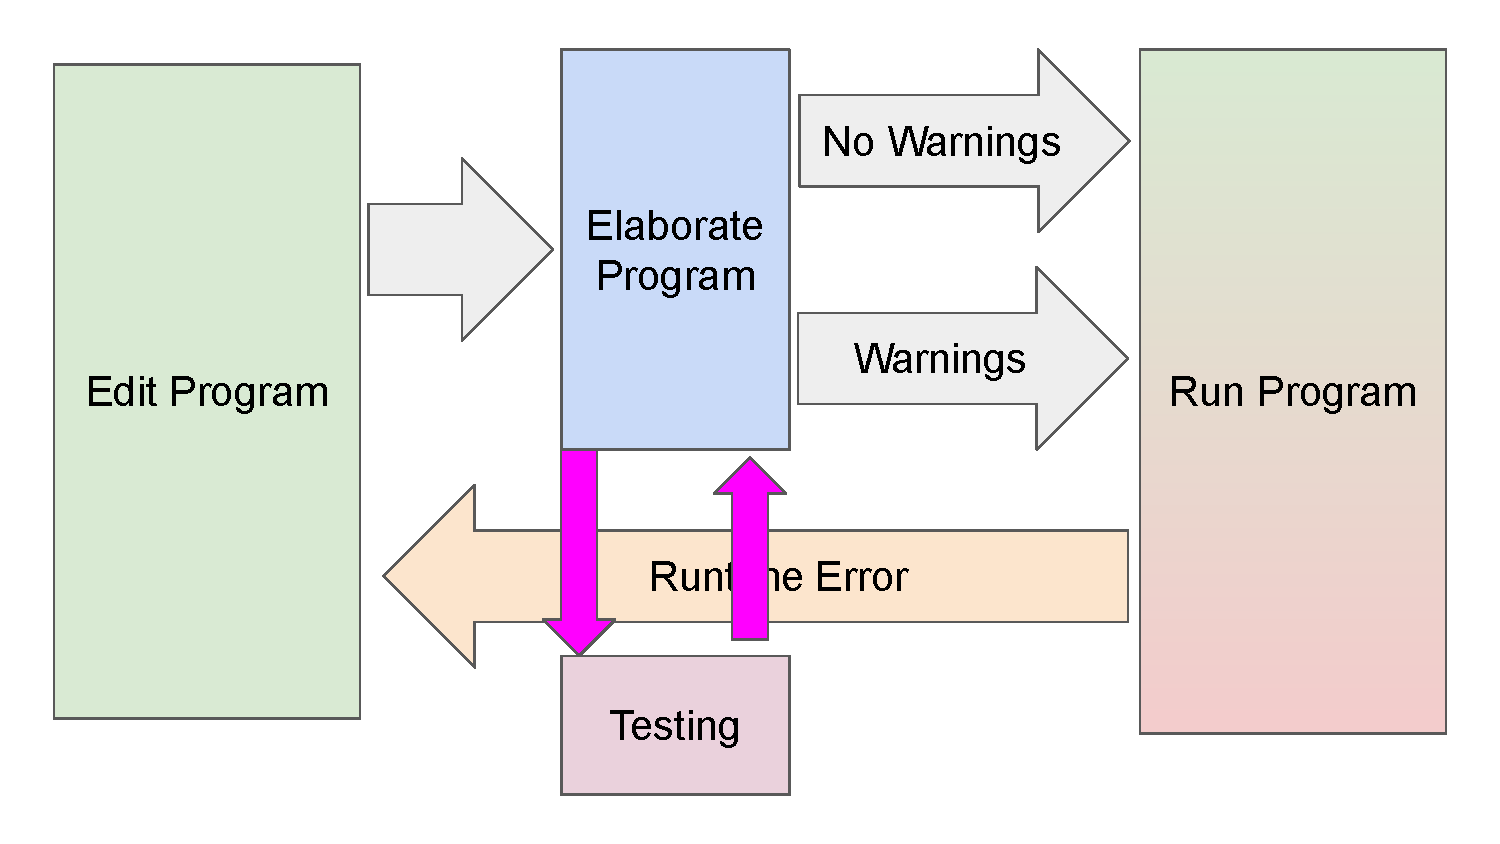
\includegraphics[width=5in]{fig/best-workflow.pdf}
% https://docs.google.com/presentation/d/1FSXDKsZlYFDNP8f6HprCrWV7gBRyW03PmIP0KkOprIA/edit#slide=id.g11561a4b8c2_0_0
\caption{Ideal Workflow}
\label{fig:notes-workflow}
\end{figure}
 
Adding a testing system to the prototype is more complicated than originally expected, and a good theory of dependently typed testing is incomplete.
 
Given those caveats, we do have a (practical?) testing procedure and some examples that might inform future theoretical work.
 
\subsection{Observable Blame}
Since this procedure operates over the \clang{}, we must decide what constitutes a reasonable testing environment
 
A one hole context\todo{cite? other people don't?} $C[-]$ can be defined for the \clang{}s presented in this thesis.
We can say that blame is observable if $\vdash a:A$ and $\vdash C[a]:B$ and $C[a]\rightsquigarrow_{*}b$ and $b\,\Blame{}_{\ell, \,o}$ for some $\ell \in lables\left(a\right)$ but $\ell \notin lables\left(C[-]\right)$\footnote{
 Even here it is questionable which specific reduction rule to use (I suspect \cbv{} would make the most sense for the implementation) and if the context should be limited to terms that elaborate from the \slang{} or all well cast terms (I use all well cast terms for convenience).
}.
 
This error observability is semi-decidable in general (by enumerating all well typed syntax).
But testing every context is infeasibly inefficient, especially if we try to synthesize open ended types, like functions.
An approximate approach can build partial testing contexts based on fixing observations to test variables.
 
% These contexts are correct up to some constraint.\todo{??}
 
\subsection{Test Environment}
The syntax for a test environment is listed in \Fref{sym-env-obs}.
The clause allows a cast context that is intended to contain data definitions for the term under test.
We can declare test variables of type ($\star$) of partial function type and partial data type.
We call them partial because they immediately defer to other test variables.
The syntax allows functions to assign an output test variable to any input.
The last 3 rules support data which as usual complicates things far more than you might expect.
Since we use endpoints to handle data, we will need to handle them symbolically, they turn out to act like constraints that the testing environment should respect.

\begin{figure}
\begin{tabular}{lcll}
\multicolumn{4}{l}{test variables,}\tabularnewline
\multicolumn{4}{l}{$X$, $Y$, $F$, $x$, $y$, $f$, $p$, $q$}\tabularnewline
\multicolumn{4}{l}{environment,}\tabularnewline
$I$ & $\Coloneqq$ & $\varGamma$ & context (to hold data definitions)\tabularnewline
  & $|$ & $I,X:\star$ & \tabularnewline
  & $|$ & $I,X\Rightarrow\star$ & \tabularnewline
  & $|$ & $I,X\Rightarrow\left(x:Y\right)\rightarrow Fx$ & \tabularnewline
  & $|$ & $I,f:\left(z:A\right)\rightarrow B$ & \tabularnewline
  & $|$ & $I,fa\Rightarrow y$ & \tabularnewline
  & $|$ & $I,X\Rightarrow D_{\Delta}\overline{x}$ & \tabularnewline
  & $|$ & $I,x\Rightarrow\left(d_{\Delta\rightarrow D\overline{A}}\overline{y}\right)::D\overline{p}$ & \tabularnewline
  & $|$ & $I,p:a\approx_{q}b$ & \tabularnewline
\multicolumn{4}{l}{Environmental Reduction,}\tabularnewline
\multicolumn{4}{l}{$I\vdash  a:A\ \vartriangleright b:B$}\tabularnewline
\end{tabular}

\caption{Test Environment}
\label{fig:sym-env-obs}
\end{figure}

Some abbreviations are listed in \Fref{sym-env-obs-abbiv}.
The syntax is presented to encourage the use of fresh variables, but these variables will be collapsed into more readable examples.

\begin{figure}
  \begin{tabular}{lcl}
  $fa\Rightarrow g,ga'\Rightarrow h$ & written & $f\,a\,a'=h$\tabularnewline
  $X\Rightarrow\left(x:Y\right)\rightarrow\star,Y\Rightarrow a$ & written & $X\Rightarrow\left(x:a\right)\rightarrow\star$\tabularnewline
  $X\Rightarrow\left(x:Y\right)\rightarrow Fx,Y\Rightarrow a$ & written & $X\Rightarrow\left(x:a\right)\rightarrow Fx$\tabularnewline
  $f:\left(x:Y\right)\rightarrow Fx,Y\Rightarrow a$ & written & $f:\left(x:a\right)\rightarrow Fx$\tabularnewline
  ... &  & \tabularnewline
  any blamable term & written & !!\tabularnewline
  \end{tabular}\caption{Environments and Observations}
  \label{fig:sym-env-obs-abbiv}
  \end{figure}

  

These testing contexts are used with the symbolic reductions rules listed in \Fref{sym-env-Sym-red} to simplify terms under test.\todo{note the funky substitution?}
Additionally, environments can shift focus into subterm positions and apply test variables to functions (these rules are unlisted).
Finally, throught this Chapter, we will use $!!$ as a short hand for some term that contains obvous blame.

\begin{figure}
  \[
  \frac{I\vdash  c:C\vartriangleright a:A\quad x\Rightarrow b\in I}{I\vdash  c:C\vartriangleright a\left[x\coloneqq b\right]:A\left[x\coloneqq b\right]}
  \]
  
  \[
  \frac{I\vdash  c:C\vartriangleright a:A\quad xb\Rightarrow y\in I}{I\vdash  c:C\vartriangleright a\left[xb\coloneqq y\right]:A\left[xb\coloneqq y\right]}
  \]
  
  \[
  \frac{I\vdash  c:C\vartriangleright a:A\quad a\rightsquigarrow a'}{I\vdash  c:C\vartriangleright a':A}
  \]
\caption{Symbolic reduction}
\label{fig:sym-env-Sym-red}
\end{figure}
 
 
\begin{example}
  Empty Type

The ``empty'' type ($\left(x:\star\right)\rightarrow x$) can be inhabited by the \clang{} term $\lambda x\Rightarrow\star::_{\ell }x$.
According to the blame rules of \Ch{3} this term does not immediately produce blame without an input.
We can observe blame by giving the function an argument, specifically by applying a function type as input.
For instance, $(\lambda x\Rightarrow\star::_{\ell }x)(\star\rightarrow\star)\ \rightsquigarrow_{*}\ \star::_{\ell }(\star\rightarrow\star)$, which is blameable.

Our symbolic execution procedure would be able to discover that example by noting the function type $\left(x:\star\right)\rightarrow x$ and applying a test variable $x$ of type $\star$.
After normalizing it is easy to see that any $x$ of the shape $x\ \Rightarrow\ -\rightarrow-$, would cause visible blame.
\end{example}


\begin{example}
Higher Order Functions

Higher order functions can be handled similarly.
For instance if we have the \clang{} term,
\[
\lambda f\Rightarrow\star::_{\ell }(f\star) \quad : \left(\star\rightarrow\star\right)\rightarrow\star
\]
\todo{perhaps explicitly condone the retroactive ch3 syntax in ch5}
  Our symbolic execution procedure would apply a test variable $f$ of type $f:\star\rightarrow\star$.
Then to observe a blamable term, symbolic execution would partially define the behavior of $f$, $f\star\ \Rightarrow\ -\rightarrow-$.
\end{example}

  
 \begin{example}
 Dependent types, function argument
  
 In the presence of dependent types, we must also consider blameable terms embedded in type formers.
 For instance, $!!\rightarrow\star\quad:\star$, can observe an error by inspecting its input, which would correspond to the context $\left(\left(\lambda x\Rightarrow x::\star\right)::[!!\rightarrow\star]::\left(\star\rightarrow\star\right)\right)\star\rightsquigarrow_{*}\star::[!!]::\star$.
 Which is blamable by the rules of \ch{3}.
\end{example}
\todo{Some examples of data}

The syntax of this system will be able to uncover every instance of observable blame.
Since it has the data definitions it needs for the term's pattern matching and every unlisted data type can be simulated by a church like encoding.
However it will also uncover many unobservable instances of blame.

Here are some additional constraints that can be applied to test environments:

\begin{itemize}
  \item $\Gamma$ holds only the well formed data definitions, for the data related to the inspected term.
  \item Variables, assignments, and paths are type and endpoint correct (with suitable extensions to the endpoint system that supports test environments).
  \item Test paths are blameless.
  \item Observably different outputs must come from observably different inputs (in the case of dependent function types, the argument should be considered as an input).
  \item Test variables are always fresh.
  For instance, $f:\Nat{}\rightarrow\Nat{},f2\Rightarrow x,f3\Rightarrow x$ would not be allowed since $f2=f3$ and is over specified.
\end{itemize}
We will call an environment where these constraints hold plausible.

Together these constraints comprise a decent testing procedure because:
\begin{itemize}
\item Can guide toward the labels of interest.
For instance, we can move to labels that have not yet observed a concrete error.
Terms without labels can be skipped entirely.
\item Can choose assignments strategically avoiding or activating blame as desired.
\item Since examples are built up partially the partial contexts can avoid introducing their own blame by construction.
\item Handle higher order functions, recursions, and self reference gracefully.
For instance, the equations $f: \Nat{} \rightarrow \Nat{}$, $f\left(f\,0\right)\Rightarrow 1$ and $f\left(3\right)\Rightarrow 3$ can be in the context if there is an assignment that implies $f\,0\neq3$
\end{itemize}
  
  
  
 However even plausible environments can flag blame that is not observable,
 \begin{itemize}
 \item
 Since there is no way for a term within the \clang{} to ``observe'' a distinction between some type formers, plausible environments cannot always be realized back to a term that would witness the bad behavior.
 For instance, the environment $F:\star\rightarrow\star,F\,\star \Rightarrow \star\rightarrow\star,F\,\left(\star\rightarrow\star\right) \Rightarrow \star$
  % , which might be needed to explore the term with casts like $\lambda F\Rightarrow...::\star::F\left(\star\rightarrow\star\right)......::\left(\star\rightarrow\star\right)::F\,\star\ :\left(\star\rightarrow\star\right)\rightarrow...$,
  will not correspond to an observable instance of blame, since there is no tem $F$ that can be constructed with those properties.
 In this way the test environment can make stronger observations than the \clang{}.
 The environment reflects a term language that has a type case construct\todo{cite}.
 % \todo[inline]{add non termination as a source of unrealizability}
 % \item
 % Additionally, the test procedure may observe \cbn{} behavior even with a \cbv{} reduction.
 % For instance, the procedure outlined above would allow $!!$ to be reached in $\left(\lambda xf\Rightarrow f(!!)\right)loop\quad:\star\rightarrow\star$ even though there is no context that would allow this to cause blame.
 % \todo{ins't as crisp an example as I would like}
 \item
 A version of parallel-or can be specified by the assignment context even though such a term is unconstructable in the language, $por:\Bool{}\rightarrow\Bool{}\rightarrow\Bool{},por\ loop\ \True{} \Rightarrow  \True{}, por\ \True{} \ loop \Rightarrow \True{},por\ \False{}\ \False{} \Rightarrow  \False{}$.
 Here all assignments are well typed, and each output can be differentiated by a different input.
\todo{G. Plotkin, LCF considered as a programming language, Theoretical
Computer Science 5 (1977) 223\{255. as cited in https://alleystoughton.us/research/por.pdf}
\end{itemize}
  
\subsection{Related and Future Work}
 
Formalizing a complete and efficient testing procedure along these lines is still future work.
However there have been other attempts to automatically test functional code that are worth mentioning.
% A fully formal account would deal with a formal semantics of the \clang{}.
 
\subsubsection{Testing}
 
Many of the testing strategies for typed functional programming trace their heritage to \textbf{property based} testing in QuickCheck \cite{quickcheck}.
Property based testing involves writing functions that encode the properties of interest, and then randomly testing those functions.
It is only natural that some of that research has been extended to dependent types:
\begin{itemize}
\item
QuickChick\footnote{https://github.com/QuickChick/QuickChick} \cite{denes2014quickchick,lampropoulos2017generating,lampropoulos2017beginner,lampropoulos2018random}
 uses type-level predicates to construct generators with soundness and completeness properties, but without support for higher order functions.
However, testing requires building type classes that establish the properties needed by the testing framework such as decidable equality.
This is presumably out of reach of novice Coq users.
\begin{itemize}
\item
Current work in this area uses coverage guided techniques in \cite{lampropoulos2019coverage} like those in symbolic execution.
More recently Benjamin Pierce has used Afl on compiled Coq code as a way to generate counter examples\footnote{https://www.youtube.com/watch?v=dfZ94N0hS4I}\todo{review this, maybe there's a paper or draft now?}.
\end{itemize}
\item \cite{dybjer2003combining} added QuickCheck style testing to (version 1 of) Agda.
\end{itemize}
 
\subsubsection{Symbolic Execution}
 
There are likely insights to be gained from the research on symbolic execution, especially work that deals with typed higher order functions.
Symbolic evaluation is a technique to efficiently extract errors from programs.\todo{make more consistent with Marco's definition}
Usually this happens in the context of an imperative language with the assistance of an SMT solver.\todo{acronym}
Symbolic evaluation can be supplemented with other techniques and an extensive literature exists on the topic.
 
The situation described in this section is unusual from the perspective of symbolic execution:
\begin{itemize}
\item The number of blamable source positions is limited by the location tags.
Thus the search in this section is blame guided, rather than coverage guided.
\item The language is dependently typed.
Often the languages studied with symbolic execution are untyped or simply typed.
\item The language in this section needs higher order functions.
Often the research in this area focuses on base types that are efficiently handleable with an SMT solver, such as integer arithmetic.
\end{itemize}
This limits the prior work to relatively few papers
\begin{itemize}
\item
A symbolic execution engine for Haskell is presented in \cite{10.1145/3314221.3314618}, but at the time of publication it did not support higher order functions.
\item
A system for handling higher order functions is presented in \cite{nguyen2017higher}, however the system is designed for Racket and is untyped.
Additionally it seems that there might be a state space explosion in the presence of higher order functions.
\item \cite{10.1007/978-3-030-72019-3_23} extended and corrected some issues with \cite{nguyen2017higher}, but still works in a untyped environment.
The authors note that there is still a lot of room to improve performance.
\item Closest to the goal here, \cite{lin_et_al:LIPIcs:2020:12349} uses game semantics to build a symbolic execution engine for a subset of ML with some nice theoretical properties.
\item An early version of the procedure described in this section was presented as an extended abstract in \cite{extendedabstract}.
However conjectures made in that preliminary work were false (the procedure would flag unreachable errors, in the sense described above).
% The underlying languages has improved substantially since that work.
\end{itemize}
The appearance of $por$ hints that the approach presented here could be revised in terms of games semantics.
Though a dependently typed game semantics also seem to have a number of unanswered questions, that correspond roughly to the issues listed above.
Though game semantics for dependent types is a complicated subject in and of itself, and has only begun to be studied in \cite{VAKAR2018401}.
\todo{System F game semantics}

% Additionally it seems helpful to allow programmers to program their own solvers that could greatly increase the search speed.
% Some preliminary work is done in \cite{VAKAR2018401}, though there language is not full spectrum and they use definitional equality to characterize observability.

\todo[inline]{
  Marco's recommended citaion!
}